%!TEX root = ../main.tex
% Chapter Template


\chapter{Latent Behaviours} % Main chapter title
\label{ch:LatentBehaviours} % Change X to a consecutive number; for referencing this chapter elsewhere, use \ref{ChapterX}
\todo[inline]{Find a suitable quote?}
\begin{quote} 
%If you only do what you can do, you will never be more than what you are now.
"As you adequately put, the problem is choice. But we already know what you are going to do, don't we?" -- The Architect.
\end{quote} 

\section{Introduction}
\todo[inline]{Give an interesting motivational example: What is the notion of latent behaviour? Why do we care about them? How is it useful to study them?}
The objective of this section is to explain the commutative diagram presented in Figure~\ref{fig:TheArrow}. This diagram, which we refer to as ``The Arrow of Latent Behaviours,'' illustrates how spatial and behavioural transformations affect the behaviour of an $F$-coalgebra $(X,c)$ by changing the behaviour map from $!_c$ to $!_{b\circ c\circ m}$. 

\begin{figure}[h]
        \centering
        \begin{tikzcd}[column sep=1.75cm, row sep=1cm]
            &\sigma F
                \arrow[dr,swap,"\Delta^m_b"']
            &
            \\ 
            X  
                \arrow[dd,"c"] 
            & X
                \arrow[l, swap, "m"]
                \arrow[u, "!_{c}"]
                \arrow[r,dotted, swap, "!_{b\circ c\circ m}"]
            &\sigma F 
                %\arrow[dd, "\simeq","\omega"']
                \arrow[dd, "1"]
                \arrow[dr, "\textbf{id}"]
            \\
            &&&\sigma(F)
            \\
            F(X)     
                \arrow[r, swap, "b"]
            &F(X)
                \arrow[d, swap, "F(!_{c})"]
                \arrow[r, dotted, "F(!_{b\circ c\circ m})"] 
            &
            F(\sigma F)
                %\arrow[ur, swap, "\omega^{-1}"]
                \arrow[ur, swap, "1^{-1}"]
            \\
            &F(\sigma F)
                \arrow[ru, swap, "F(\Delta^m_b)"]
            &
        \end{tikzcd}
        \caption{``The Arrow of Latent Behaviours.'' This commutative diagram summarises the effect of spatial and behavioural transformations over the $F$-coalgebra $(X,c)$, respectively modelled by $m$ and $b$: the behaviour map changes from $!_c$ to $!_{b\circ c\circ m}$. Latent behaviour analysis assumes $b=\id$.}
        \label{fig:TheArrow} 
    \end{figure}

\section{Motivation: Fault Injection via Carrier Transformations}
\todo[inline]{Small intro to faulty systems. You should have mentioned already somewhere in the intro that there are two ways to mutate the behaviour of a system in the coalgebra world: by transforming the carrier or by transforming the co-carrier. We only study transformations of the carrier.}
\todo[inline]{I feel like we are missing some stuff? How are we going to structure the introduction?}

Consider the automaton shown in Figure~\ref{fig:ExampleLatent}, which recognises the language of sequences of zeroes and ones that end in two consecutive ones; i.e., the language $(0+1)^*11$. 
This automaton is defined by the tuple $(\vec{X},\vec{x}_0,\delta,F)$, where the carrier is $\vec{X}=2\times2$, the initial state is $\vec{x}_0\colon1\rightarrow \vec{X}$ with $\vec{x}_0(\star)=(0,0)$, the transition function $\delta\colon \vec{X}\rightarrow 2\rightarrow\vec{X}$ is defined for $\vec{x}\in \vec{X}$ and $i \in 2$ by $\delta(\vec{x})(i)=(i,\vec{x}[0]),$ and the characteristic predicate of the set of accepting states is $F\colon\vec{X}\rightarrow 2$, where $F(1,1)=1$ and $F(x,y)=0$ otherwise; i.e. $(1,1)$ is the only accepting state. This automaton is not minimal, since the states $(0,0)$ and $(0,1)$ are bisimilar.

\begin{figure}[t]
    \centering
    \begin{tikzpicture}
        \node[state,initial] (00) {$(0,0)$};
        \node[state, below right of=00] (01) {$(0,1)$};
        \node[state, above right  of=00] (10) {$(1,0)$};
        \node[state, accepting, below right of=10] (11) {$(1,1)$};
        \draw (00) edge[bend left, above] node{1} (10)
        (00) edge[loop above] node{0} (00)
        (01) edge[bend left, left] node{1} (10)
        (01) edge[bend left, above] node{0} (00)
        (10) edge[bend left, above] node{1} (11)
        (10) edge[bend left, right] node{0} (01)
        (11) edge[loop above] node{1} (11)
        (11) edge[bend left, above] node{0} (01)
        ;\end{tikzpicture}
    \caption{An automaton which recognises the language $(0+1)^*11$.}
    \label{fig:ExampleLatent}
\end{figure}

Now, %assume that the programmer is malicious, and they purposely 
consider a symmetry in the state space which maps $(a,b)$ to $(\lnot a, \lnot b)$. This transformation models some fault which could be introduced by a malicious programmer. Formally, %the programmer applies a 
we define the transformation $m\colon \vec{X}\rightarrow\vec{X}$ for $\vec{x}\in \vec{X}$ by $m(\vec{x})=(\lnot \vec{x}[0],\lnot \vec{x}[1])$. 
State transformations are applied before behaviour is computed; thus, if the current state is $\vec{x}=(a,b)$, when we intend to check whether $\vec{x}$ is accepting, we instead check whether $(\lnot a, \lnot b)$ is accepting, and when we intend to compute $\delta(i)(\vec{x})$, we instead compute $\delta(i)(\lnot a, \lnot b)$. 

\begin{figure}[t]
    \centering
\begin{tikzpicture}
    \node[state, initial, accepting] (00) {$(0,0)$};
    \node[state, below right of=00] (01) {$(0,1)$};
    \node[state, above right  of=00] (10) {$(1,0)$};
    \node[state, below right of=10] (11) {$(1,1)$};
    \draw (00) edge[bend right, above] node{1} (11)
    (00) edge[bend right, above] node{0} (01)
    (01) edge[bend right, above] node{1} (11)
    (01) edge[loop below] node{0} (01)
    (10) edge[loop above] node{1} (10)
    (10) edge[bend right, above] node{0} (00)
    (11) edge[bend right, above] node{1} (10)
    (11) edge[bend right, above] node{0} (00)
    ;\end{tikzpicture}
\caption{Automaton that models the faulty implementation.}
\label{fig:Transformed}
\end{figure}
Figure~\ref{fig:Transformed} shows a model of the faulty system. This automaton recognises the language of sequences of zeroes and ones that are either empty or end in 10; i.e., $\varepsilon+(0+1)^*10$. 
Before we explain why the automaton in Figure~\ref{fig:Transformed} models the faulty system, we can test if this system recognises sequences $\varepsilon+(0+1)^*10$. %$(0+1)(0+1)^*$. 
To do so, let us consider pairs of states $[\vec{x},\vec{y}]$ where $\vec{x}=(x_1,x_2)$ and $\vec{y}=(y_1,y_2)$ such that the pair $\vec{x}$ follows the original behaviour, i.e., without faults, while $\vec{y}$ follows the faulty behaviour. 
The initial state is $[(0,0),(0,0)]$. %, since $(1,1)$ replaces $(0,0)$ due to the fault. 
The trace of the sequence $00$ is 
\begin{align*}
   [(0,0),(0,0)]&\xrightarrow{\id\times m}[(0,0),(1,1)]\xrightarrow{\delta(0)\times\delta(0)}[(0,0),(0,1)]\\
   &\xrightarrow{\id\times m}[(0,0),(1,0)]\xrightarrow{\delta(0)\times\delta(0)}[(0,0),(0,1)]\\
   &\xrightarrow{\id\times m}[(0,0),(1,0)]\xrightarrow{F\times F}[0,0],
\end{align*}
so $00$ is rejected by both automata. %Note that $\delta(0)(1,1)=(0,1)$, but since $(1,0)$ replaces all read uses of $(0,1)$, we apply the fault directly. 
Now, if we receive the sequence $10$, the resulting state trace is 
\begin{align*}
    [(0,0),(0,0)]&\xrightarrow{\id\times m}[(0,0),(1,1)]\xrightarrow{\delta(1)\times\delta(1)}[(1,0),(1,1)]\\
   &\xrightarrow{\id\times m}[(1,0),(0,0)]\xrightarrow{\delta(0)\times\delta(0)}[(0,1),(0,0)]\\
   &\xrightarrow{\id\times m}[(1,0),(1,1)]\xrightarrow{F\times F}[0,1];
\end{align*}
the faulty automaton accepts $10$, but the original automaton does not. 
The trace of the sequence $11$ is 
\begin{align*}
    [(0,0),(0,0)]&\xrightarrow{\id\times m}[(0,0),(1,1)]\xrightarrow{\delta(1)\times\delta(1)}[(1,0),(1,1)]\\
   &\xrightarrow{\id\times m}[(1,0),(0,0)]\xrightarrow{\delta(1)\times\delta(1)}[(1,1),(1,0)]\\
   &\xrightarrow{\id\times m}[(1,1),(0,1)]\xrightarrow{F\times F}[1,0],
\end{align*}
so $11$ is accepted by the original automaton, but rejected by the faulty automaton. 
For the sequence $110$, the resulting state trace is 
\begin{align*}
    [(0,0),(0,0)]&\xrightarrow{\id\times m}[(0,0),(1,1)]\xrightarrow{\delta(1)\times\delta(1)}[(1,0),(1,1)]\\
   &\xrightarrow{\id\times m}[(1,0),(0,0)]\xrightarrow{\delta(1)\times\delta(1)}[(1,1),(1,0)]\\
   &\xrightarrow{\id\times m}[(1,0),(0,1)]\xrightarrow{\delta(0)\times\delta(0)}[(0,1),(0,0)]\\
   &\xrightarrow{\id\times m}[(0,1),(1,1)]\xrightarrow{F\times F}[0,1];
\end{align*}
the faulty automaton accepts $110$, but the original automaton does not. Finally, the original automaton rejects the empty sequence $\varepsilon$, but the faulty automaton accepts it, since 
\begin{align*}
    [(0,0),(0,0)]\xrightarrow{\id\times m}[(0,0),(1,1)]\xrightarrow{F\times F}[0,1].
\end{align*} 

% The map $m$ pairs each state with its corresponding faulty representation. %If there were no faults, the map $m$ would be the identity map. 
% The fault forces the state $(0,0)$ to behave like its image under $m$, i.e., the behaviour of $(0,0)$ in the faulty system should behave like $(1,1)$. Similarly, the state $(1,1)$ should behave $(0,0)$. 
%(We can alternatively see the function $m$ as a bad abstraction from the implementation.)

%There are now two final states: $(1,1)$ and $(0,1)$ since both states are preimages of $(1,1)$ under $m$.
We obtain the automaton shown in Figure~\ref{fig:Transformed} by ``copying'' the original behaviour from images of $m$ to their preimages. Figure~\ref{fig:ExampleWithFaults} shows this procedure for $(0,0)$ and $(1,1)$. This includes copying the behaviour under $\delta$ and under $F$. 

We preserve the initial state because $\vec{x}_0$ is a selection/construction/algebraic operation, not a behavioural/semantic/coalgebraic operation. We do not apply transformations to the results of algebraic operations to avoid aggregating the transformation erroneously due to composition of algebraic and coalgebraic operations. Consider the followign: the initial state $\vec{x}_0$ is of type $1\rightarrow\vec{X}$ which is algebraic, so the only way to apply $m$ to $\vec{x}_0$ is by composing it on the left, i.e., $m\circ \vec{x}_0(\star)$. Checking if the initial state is accepting in the original automaton corresponds to the expression $(F\circ\vec{x}_0)(*)$; however, the expression
\begin{align*}
    (F\circ m)\circ (m\circ\vec{x}_0)(\star)= (F\circ m)(1,1)=F(0,0)=0,
\end{align*}
applies $m$ twice, and it fails to properly check if the initial state of the faulty automaton is final. Instead, the correct expression is 
\begin{align*}
    (F\circ m)(\vec{x}_0)= (F\circ m)(0,0)=F(1,1)=1.
\end{align*}
% In other words, since $m(0,0)=(1,1)$, we copy the original behaviour of $(1,1)$ and we give it to $(0,0)$, including that $(1,1)$ is an accepting state; similarly, since $m(1,1)=(0,0)$ we copy the original behaviour of $(0,0)$ to $(1,1)$. 
% We do not change the initial state because 

\begin{figure}[t]
    \centering
    \begin{tikzpicture}
        \node[state] (00) {$(0,0)$};
        \node[state, below right of=00] (01) {$(0,1)$};
        \node[state, above right  of=00] (10) {$(1,0)$};
        \node[state, below right of=10] (11) {$(1,1)$};
        \draw 
        (00) edge[above, bend left, dashed,color=gray] node[color=lightgray]{1} (10)
        (00) edge[loop above, dashed,color=gray] node[color=lightgray]{0} (00)
        % (01) edge[bend left, dashed,color=gray] (10)
        % (01) edge[bend left, below, dotted, color=gray](00)
        % (10) edge[bend left, dashed, color=gray] (11)
        % (10) edge[bend left, right, dotted, color=gray] (01)
        (11) edge[loop above, dashed, color=gray] node[color=lightgray]{1} (11)
        (11) edge[bend left, below, dashed, color=gray]node[color=lightgray]{0} (01)
        %Mutation Arrows
        (00) edge[color=gray, dotted] (11) 
        % (01) edge[color=red,dotted]  (10)
        % (10) edge[color=red, dotted]  (01)
        (11) edge[color=gray, dotted] (00)
        %New arrows
        (00) edge[bend right, below,color=red] node{0} (01)
        (00) edge[bend right, below,color=red] node{1} (11)
        (11) edge[bend right, above,color=red] node{0} (00)
        (11) edge[bend right, above,color=red] node{1} (10)
        % (11) edge[above] node{1} (1,0)
        % (11) edge[bend right, above] node[near start]{0} (00)
        ;\end{tikzpicture}
    \caption{Composition of the fault $m$ and the original behaviour for the states $(0,0)$ and $(1,1)$. The dotted, gray, bidirectional arrow in the centre models the effect of the fault $m$. The original behaviours appear as dashed, grey lines. The behaviour which results from the composition appears as solid, red lines.}
    \label{fig:ExampleWithFaults}
\end{figure}
We say that the faulty system is \emph{latent} with respect to the original system, since the application of the transformation $m$ reveals it, and $m$ is not the identity function. 
We cannot model every fault using transformations of the state space. The set of behaviours that we can obtain is limited; e.g., the behaviour of an automaton that accepts every sequence cannot be transformed by just transforming the state space. 
To transform an automaton which accepts all sequences into one that can reject some or all, we need a transformation of the \emph{behaviour}. 
Those transformations correspond to the arrow $F(X)\xrightarrow{b}F(X)$ in Figure~\ref{fig:TheArrow}. 
\todo[inline]{the final coalgebra is the place where spatial, behavioural, and coalgebras meet. Spatial transformations abstract a behaviour acting concurrently with the one we are currently studying, and that's why they are interesting to study.}
%However, systems revealed by transformations of type $F(X)\xrightarrow{b}F(X)$ are not latent by definition. %In this thesis, we are interested in seeing how far we can go with just carrier transformations; i.e., with latent behaviours.

We now present a general treatment for carrier transformations and latent behaviours in the context of $F$-coalgebras. 

\todo[inline]{Remark eventually that we cannot model every malicious behaviour of the programmer, only those that affect state, not functionality.}
\section{Latent $F$-coalgebras}
\todo[inline]{First write about the coalgebras and how they connect behaviours... then come back to this section.}
Coalgebras offer an interesting perspective for the study of systems. Given an $F$-coalgebra $(X,c\colon X\rightarrow F(X))$, each state $x\in X$ has an associated behaviour $c(x)\in F(X)$. In this section, we study the effect of a state transformation $m\colon X\rightarrow X$ over the $F$-coalgebra $(X,c)$. 

In terms of types, we can always compose the function $c$ with any carrier transformation $m$; the composition $c \circ m\colon X\rightarrow F(X)$ exists and is well defined. However, the behaviour of elements might be greatly affected. In particular, states which are bisimilar under $c$ might no longer be bisimilar under $c \circ m$. If $m$ preserves bisimilarity, then we say that $m$ is \emph{(behaviourally) consistent}.

\begin{definition}[Consistent Spatial Transformations]
Given an $F$-coalgebra $(X,c)$, any function of type $m\colon X\rightarrow X$ is a \emph{spatial transformation}. %A transformation $m\colon X \rightarrow X$ has \emph{finite support} iff $m(x)\neq x$ only for a finite number of $x\in X$. We denote the set of finitely supported transformations by $X^X_\omega$. 
A spatial transformation $m$ is \emph{(behaviourally) consistent} if and only if, whenever $x\sim_c y$, then $m(x)\sim_{c} m(y)$, for all $x,y \in X$. %We denote the set of consistent transformations by $X^X|_\sim$. %
\end{definition}
Henceforth, we consider only minimal systems, unless explicitly mentioned otherwise. 
\begin{corollary}
    If $(X,c)$ is a minimal $F$-coalgebra, then every spatial transformation %$m\colon X\rightarrow X$ 
    is consistent. 
\end{corollary}
A transformation function $m\colon X\rightarrow X$ changes the normal behaviour of $\mathbb{X}$, and it reveals the \emph{latent coalgebra of $\mathbb{X}$ under $m$}. 
\begin{definition}[Latent Coalgebra]
Given an $F$-coalgebra $\TheCoalgebra=(X,c)$ and a transformation $m$, the \emph{latent coalgebra of $\mathbb{X}$ under $m$} is $(X,c\circ m)$. 
% \begin{align}
%     \mathbb{X}\circ m\triangleq(X,{(o\circ m, \delta\circ m })).
% \end{align}
The function $\TheLatentBehaviourOfIn{\cdot}{m}{c}\colon X\rightarrow \sigma F$ defines the \emph{latent behaviour} under $m$. The homomorphism $\TheLatentBehaviourOfIn{\cdot}{m}{\mathbb{X}}$ corresponds to the semantic mapping of the $F$-coalgebra $(X,c\circ m)$; that is, for $x\in X$, 
\begin{align}
\TheLatentBehaviourOfIn{x}{c}{m}\triangleq\TheBehaviourOfIn{x}{{c\circ m}}
\end{align} 

A LBA of an $F$-coalgebra $(X,X\xrightarrow{c} F(X))$ is the study of the effect that a spatial transformation $m\colon X\rightarrow X$ has over the behaviour of states in $X$, i.e., the shift in semantics from $c$ to $c\circ m$. It is also possible to change behaviour by composing $c$ with a \emph{behaviour transformation} $b\colon F(X)\rightarrow F(X)$ on the left. Both $(X,b\circ c\colon X\rightarrow F(X))$ and $(X,b\circ c\circ m\colon X\rightarrow F(X))$ are $F$-coalgebras, since the type requirement is satisfied. The effect of behaviour transformations in arbitrary systems are beyond the scope of this work. Nevertheless, there are systems where behaviour transformations and spatial transformations coincide: final $F$-coalgebras.

\subsection{Latent Behaviours of Final $F$-coalgebras}
A final $F$-coalgebra $(\sigma F, 1)$ has a behaviour function $1\colon \sigma F \rightarrow \sigma F$ that is an isomorphism. Since $\sigma F \simeq F(\sigma F)$, it naturally follows that 
\begin{align}
    \sigma F\rightarrow \sigma F \simeq \sigma F\rightarrow F(\sigma F) \simeq F(\sigma F)\rightarrow F(\sigma F).    
\end{align}
In other words, in the carrier of the final $F$-coalgebra, spatial transformations ($\sigma F\rightarrow \sigma F$), behavioural transformations ($F(\sigma F)\rightarrow F(\sigma F)$) and $F$-coalgebras ($\sigma F\rightarrow F(\sigma F)$) are in a one-to-one correspondence. 

Intuition tells us that $1\colon \sigma F \rightarrow F(\sigma F)$ should correspond to $\id_{\sigma F}\colon \sigma F\rightarrow \sigma F$ and should correspond to $\id_{F(\sigma F)}\colon F(\sigma F)\rightarrow F(\sigma F)$. The general form is given by the following proposition.
\begin{proposition}
    For every $F$-coalgebra $(\sigma F, c)$, there are transformations $m\colon \sigma F\rightarrow \sigma F$ and $b\colon F(\sigma F)\rightarrow F(\sigma F)$ such that the diagram in Figure~\ref{fig:FinalEquivalence} commutes.
\end{proposition}
\begin{proof}
    Since $1\colon \sigma F\rightarrow F(\sigma F)$ is an isomorphism, by taking $m=1^{-1}\circ c$ and $b=c\circ 1^{-1}$, the diagram in Figure~\ref{fig:FinalEquivalence} commutes.
\end{proof}
\begin{corollary}
    Every $F$-coalgebra $(\sigma F, c)$ is a latent coalgebra of $(\sigma F, 1)$ under some spatial transformation $m\colon \sigma F\rightarrow \sigma F$.
\end{corollary}
This property is exclusive to the carrier of the final coalgebra, because of the reversibility of the final map $1$, which formalises a correspondence between state and behaviour. For an arbitrary $F$-coalgebra $(X,c)$, only some latent $F$-coalgebras can be revealed by spatial transformations $m\colon X\rightarrow X$, and such a set of revealed behaviours is determined by the available \emph{gadgets}.

\section{Gadgets}
In the context of return-oriented programming~(\cite{ROP}), a \emph{gadget} is a code snipped that is part of the original program, and it is exploited by attackers to hijack the control flow once they affect the return addresses of functions. In the context of LBA, given an $F$-coalgebra $(X,c)$, if $c$ defines the program, then the set of \emph{gadgets} we can use to change the behaviour of the system are the behaviours in $F(X)$ that are available through $c$.
\begin{definition}[Gadgets]
    Let $\mathbb{X}=(X,c)$ be an $F$-coalgebra; %, and $m\colon X\rightarrow X$ be a spatial transformation
    we define the set of \emph{gadgets of $\mathbb{X}$} by $c(X)$. 
\end{definition}
\begin{corollary}
    In minimal systems, there is one gadget per state.
\end{corollary}
A gadget is a behavioural building block that we can exploit via spatial transformations. The intuition is to think of gadgets as just functions that take one state and produce another state and an observation.
Gadgets respond differently to different inputs (which, in this case, are states).

%Depending on the carrier we choose, we can give more flexibility to the generation of latent coalgebras.%The premise is then the following: if the behaviour of a system is completely determined by its current state, then transforming the current state yields a new behaviour. 

In the following, we work on arbitrary $F$-coalgebras $(X,c)$ and only consider spatial transformations to

\begin{figure}[t] 
    \centering
    \begin{tikzcd}[column sep=1.5cm, row sep=1.5cm]
         \sigma F
            \arrow[r,"m"]
            \arrow[dr,"c"]
            \arrow[d,"1"']
        &\sigma F
            \arrow[d,"1"]
        \\
         F(\sigma F)
            \arrow[r,"b"']
        &F(\sigma F)
            %\arrow[u,"1^{-1}"']
    \end{tikzcd}
    \caption{Every $F$-coalgebra $(\sigma F, c)$ can be revealed from the final coalgebra $(\sigma F,1)$ by means of a transformation $m$ or a transformation $b$. In other words, it suffices to use spatial transformations $m$ and the final $F$-coalgebra to reveal all $F$-coalgebras of $\sigma F$, so behavioural transformations $b$ are unnecessary.}
    \label{fig:FinalEquivalence} 
\end{figure}


% \paragraph{Space-Time Duality} 
% We now define the set $m(X)\triangleq\{m(x)\ |\ x\in X\}$. We define a dynamical system $(m(X),m\circ c\colon m(X)\rightarrow m(X))$, whose associated set of behaviours is $(m\circ c)_{m(X)}^\infty$.

% \begin{figure}[t]
%     \centering
%     \begin{tikzcd}%[column sep=1.75cm, row sep=1cm]
%         X\times X
%             \arrow[d,swap,"\id\circ \fst"]
%             \arrow[r,swap,"m\circ \snd"']
%         & X
%             \arrow[d,swap,"c"']
%         \\ 
%         X
%             \arrow[r,swap,"c\circ m"]
%         &  F(X)
%     \end{tikzcd} 
%     \caption{WRONG PULLBACK IDIOT. The pullback we want is between $c$ and }
% \end{figure}

% \begin{theorem}[Fundamental Theorem of Latent-Behaviour Analysis]
%     \label{theo:Fundamental}
%     The semantic map-ping of the $F$-coalgebra $(X,c\circ m\colon X\rightarrow F(X))$ factors through the semantic mapping of the $F$-coalgerba $(m(X),c\colon m(X)\rightarrow F(m(X)))$
%     \todo[inline]{This probably needs to use bounded functors.}
% \end{theorem}
% \begin{proof}
%     The Epi-mono factorisation from Universal Coalgebra uses the kernel of homomorphisms as the quotient. Here, we replace it by $\equiv_m$, enforcing bisimilarity between $x$ and $m(x)$. Note that $\equiv_{\id}$ results in normal bisimilarity, because no enforcement takes place.

%     The transformation $m\colon X\rightarrow X$ forces the appearances of equivalence classes $\equiv_m\subseteq X\times X$ with respect to $c$, where $x_1\equiv_m x_2$ iff $m(x_1)\sim m(x_2)$, which overrides bisimilarity in $X$ with respect to $c$. The set $X/\equiv_m$ is isomorphic to $m(X)$. In other words, 
% \end{proof}

% \begin{figure}[t]
%     \centering
%     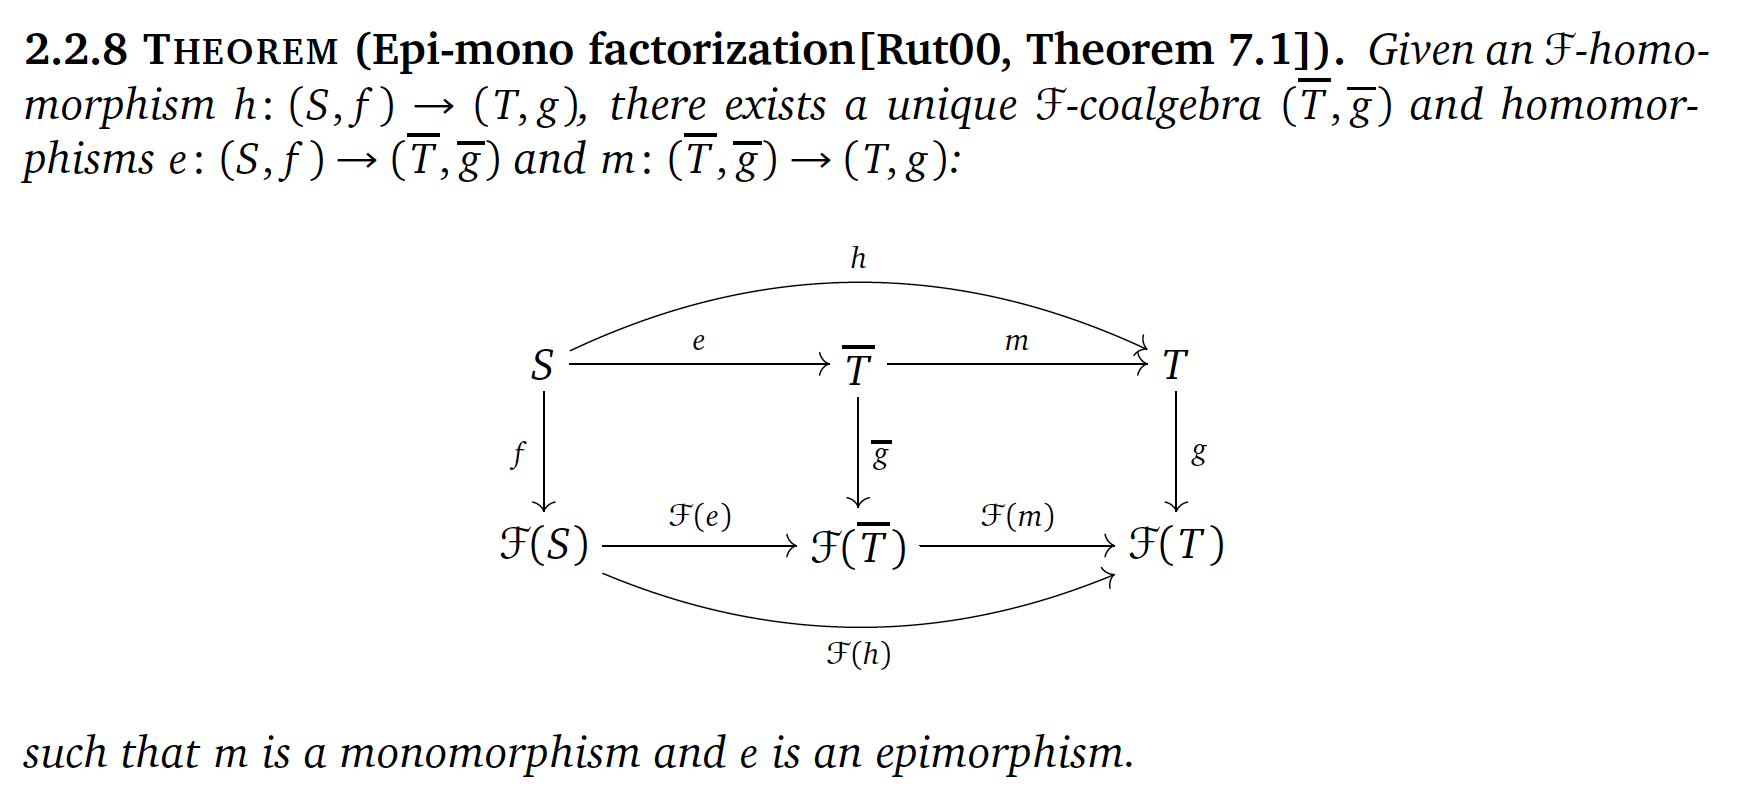
\includegraphics[width=1\textwidth]{Figures/Epi-monofactorisation.png}
%     \caption{Reason why the fundamental theorem works.}
%     \label{fig:LambdaCurves}
%     \end{figure}

% \begin{figure}[t]
%     \centering
%     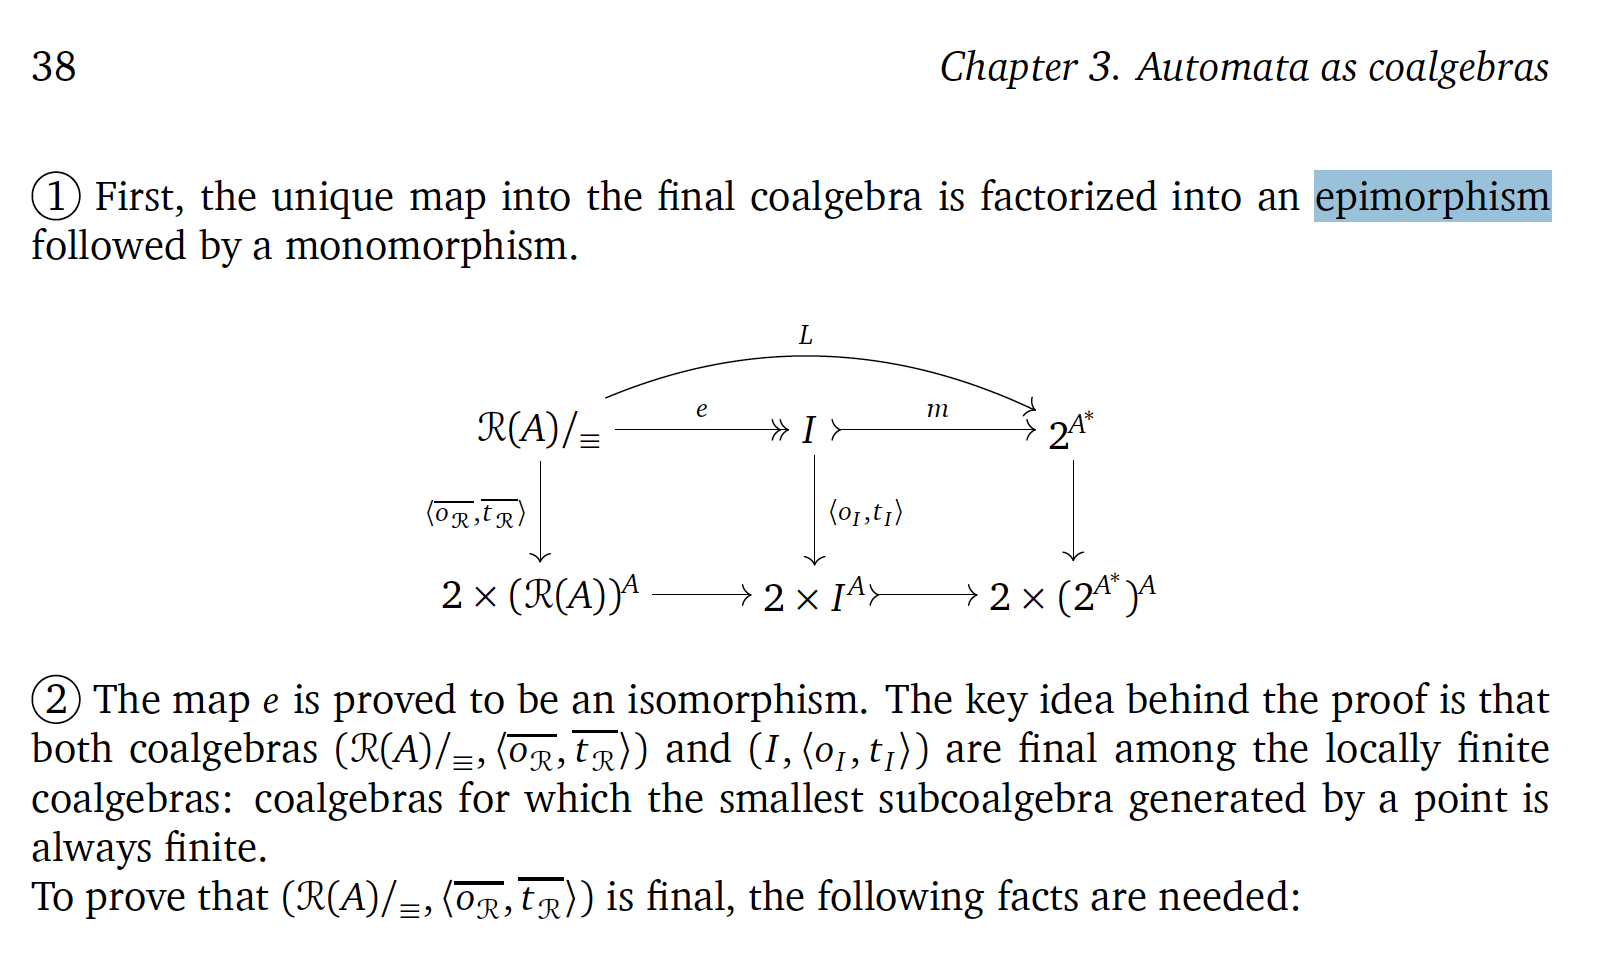
\includegraphics[width=1\textwidth]{Figures/FundamentalTheo.png}
%     \caption{Reason why the fundamental theorem works.}
%     \label{fig:LambdaCurves}
%     \end{figure}

\begin{proposition}[Behavioural Change]
For any dynamical system described by an $F$-coalgebra 
$(X,c\circ m\colon X\rightarrow F(X))$, where $m\colon X\rightarrow X$, and  $c\colon X\rightarrow F(X)$, there exists a \emph{unique} transformation function $\Delta_m\colon \sigma F\rightarrow \sigma F$ which maps $\TheBehaviourOfIn{x}{c}$ to $\TheLatentBehaviourOfIn{x}{c}{m}$, describing the \emph{behavioural change} of $x$, for all $x\in X$.
\end{proposition}
\begin{proof}
    The function $\Delta_{m}\colon \sigma F\rightarrow \sigma F$ is an $F$-coalgebra since $F(\sigma F)\simeq \sigma F$, so it has a behaviour. 
coinductively defined by 
{\color{red}
\todo[inline]{Transform this into a commutative diagram?}
\begin{align*}
    \Delta_{m}(\TheBehaviourOfIn{x}{c}) \sim_{(c \circ m)} (x)\\
    %\Delta_{m}(c^\infty_x)[1]&\triangleq c^\infty_{m(x)}[1]\\
    \Delta_{m}(c^\infty_x)[t+1]&\triangleq \Delta_{m}\left(c^\infty_{(c\circ m)(x)}\right)[t]
\end{align*}
}
\end{proof}

\section{Dynamical Systems of the $\id$ Functor}
% Theorem~\ref{theo:Fundamental} is a far stretch from the fundamental theorem of arithmetic, which states that every natural number can be decomposed into a multiplication of primes, but it follows a similar reasoning. Normally, we ignore this decomposition, so $\delta=c$ and $m=\id$. 
% \todo[inline]{It would be nice to have ``primes" here, and they may exist. They'll probably }



The \emph{fundamental theorem of latent behaviour analysis} implies the existence of unique transformation function $\Delta_m\colon X^\infty\rightarrow X^\infty$ which maps $c_{x}^\infty$ to both $\delta_{x}^\infty$ and $c_{m(x)}^\infty$ for all $x\in X$. The function $\Delta_m$ models the behavioural change induced by $m$ when applied to the $F$-coalgebra $(X,c)$. This unique function $\delta_{x}^\infty$ and $c_{m(x)}^\infty$ is 
coinductively defined by 
% \todo[inline]{BE CAREFUL HOW YOU DEFINE THE INDICES and if you want behaviours to include $x$, in coalgberas that is not very common.}
\begin{align*}
    \Delta_{m}(c^\infty_x)[0]&\triangleq (c \circ m)(x)\\
    %\Delta_{m}(c^\infty_x)[1]&\triangleq c^\infty_{m(x)}[1]\\
    \Delta_{m}(c^\infty_x)[t+1]&\triangleq \Delta_{m}\left(c^\infty_{(c\circ m)(x)}\right)[t]
\end{align*}
This definition compounds the effect of $m$ over time.
% \begin{align}
%     \Delta_m(c_{x}^\infty)\triangleq(m\circ c)_{x}^\infty
% \end{align}
% which is not a very useful definition. However, if $m$ satisfies some linearity properties, then this function $\Delta_m(c_{x}^\infty)$ can be defined (co)inductively.

For example, consider the system $(\mathbb{N},c=(+1))$ and the operator $m=(*3)$. The corresponding definition is $\Delta_{m}$ by
\begin{align*}
    \Delta_{m}(c^\infty_x)[0]&=1\\%(+1)^\infty_{2x}[1]\\
    (\Delta_{m}(c^\infty_x))[t+1]&=\Delta_{m}(c^\infty_{3x+1})[t]
\end{align*}
%This definition compounds the effect of the operator $(*2)$. 
From $(1,2,3,\ldots)=(+1)^\infty_0$, we obtain the sequence $(1,7,13,40,121,\ldots)$. 
% Now, $\Delta_{(*2)}(\omega)[0]=0$. %, so $((+1)\circ (*2))^\infty_0[0]=0$. 
% Next, $\Delta_{(*2)}(((+1)\circ (*2))^\infty_{1})[0]=1$

%$\Delta_{(*2)}(\omega)[t+1]$ since $\omega=(+1)^\infty_{(2*0)+1}$
\begin{definition}
The operator $m$ is \emph{linear with respect to $c$} if and only if
\begin{align}
    (c\circ m)^\infty_x[t]= (m \circ c)^\infty_x[t].
\end{align}    
\end{definition}

%Functorial operators are quite rare. It means that their effects do not compound over time. 
% (Linear operators have a deep relation to bialgebras of the identity functor, where $c\circ m= m\circ c $.)
% The operator $(*2)$ is not linear with respect to $(+1)$, but the operator $+3$ is. $(0,4,8,)$.

Depending on the properties of $m$ and $\Delta_m$, we might infer whether some behavioural property was preserved for all sequences, i.e., if $P(c^\infty_x)$, then $P((c\circ m)^\infty_x)$. For example, for $m=(*3)$, and $c=(+1)$, the sequence is still strictly increasing. 



%We say that thefunction $\Delta^m$ has a solution if it can be written








THe usefulness of latent behaviour analysis is that you can decompose a behaviour-defining into several components. Each of those components 



\todo[inline]{Latent coalgebras are coalgebras with the state space deformed.}
\todo[inline]{THESE DIAGRAMS ARE WRONG. THE BEH OF C CANNOT APPEAR LIKE THISOR YOU CAN GO VIA M to the end of c}
\end{definition}
\begin{figure}
    \centering
    \begin{tikzcd}[column sep=large]
        \sigma F
            \arrow[d, "\simeq","\omega"'] 
        &X
            \arrow[r, "m"]
            %\arrow[rd, "c\circ m", red]
            \arrow[l, dotted, swap,"\TheBehaviourOf{\cdot}_{c\circ m}"]
        &X 
            \arrow[r, dotted, "\TheBehaviourOf{\cdot}_c"] 
            \arrow[d, "c"] 
        & \sigma F 
            \arrow[d, "\simeq","\omega"'] 
        \\
        F(\sigma F)
        &
        &F(X) 
            \arrow[r, dotted, "F(\TheBehaviourOf{\cdot}_c)"]
            \arrow[ll, dotted, swap,"F(\TheBehaviourOf{\cdot}_{c\circ m})"]     
        &F(\sigma F)
    \end{tikzcd}
    \caption{$(X,c\circ m)$ is an $F$-coalgebra, so it has a unique $F$-homomorphism to the final $F$-coalgebra $(\sigma F, \omega)$. Geometrically, $m$ is a transformation of the state space, so some preserve certain structural properties (e.g. a permutation) while others do not (e.g. a collapsing function to some fixed $x$).}
\end{figure}
\begin{figure}
    \centering
    \begin{tikzcd}[column sep=large]
        \sigma F
            \arrow[d, "\simeq","\omega"'] 
        &&X
            \arrow[r, "m"]
            \arrow[d, "b\circ c\circ m"] 
            %\arrow[rd, "c\circ m", red]
            \arrow[ll, dotted, swap,"\TheBehaviourOf{\cdot}_{b\circ c\circ m}"]
        &X 
            \arrow[rr, dotted, "\TheBehaviourOf{\cdot}_c"] 
            \arrow[d, "c"] 
        && \sigma F 
            \arrow[d, "\simeq","\omega"'] 
        \\
        F(\sigma F) 
        &&F(X) \arrow[ll, dotted, swap,"F(\TheBehaviourOf{\cdot}_{b\circ c\circ m})"]
        &F(X) 
            \arrow[rr, dotted, "F(\TheBehaviourOf{\cdot}_c)"]
            \arrow[l, "b"]     
        &&F(\sigma F)
    \end{tikzcd}
    \caption{Latency using both $m$ and $b$ to reveal latent behaviours: $(X,b\circ c\circ m)$ is still an $F$-coalgebra, so it has a unique $F$-homomorphism to the final $F$-coalgebra $(\sigma F, \omega)$. Metaphorically, consider the function $c$ as a causal model which transforms the cause $x$ into the consequence $c(x)$; the transformation $m$ corresponds to a change of cause, while a transformation $b$ corresponds to a change of consequence. In a more concrete example, assume that we are grading a test, and $c$ is the grading rules. The value $c(x)$ is the grade assigned to the answers $x$. A transformation $m$ would correspond to changing the answers before grading, while a transformation $b$ corresponds to changing the grade after the answers have been graded. Now, if $F(X)$ is the The transformation $b$ needs not respect the properties of $c$, since it is applied after it. Thus, it would be possible to change the grade through $b$ to some value that is impossible to obtain by any possible combination of answers (i.e. for every $m$ that changes answers).}
\end{figure}
\begin{figure}
    \centering
    \begin{tikzcd}[column sep=large]
        \sigma F
            \arrow[d, "\simeq","\omega"'] 
        &X
            \arrow[r, "m"]
            %\arrow[rd, "c\circ m", red]
            \arrow[l, dotted, swap,"\TheBehaviourOf{\cdot}_{c\circ m}"]
        &X 
            \arrow[r, dotted, "\TheBehaviourOf{\cdot}_c"] 
            \arrow[d, "c"] 
        & \sigma F 
            \arrow[d, "\simeq","\omega"'] 
        \\
        F(\sigma F)
        &
        &F(X) 
            \arrow[r, dotted, "F(\TheBehaviourOf{\cdot}_c)"]
            \arrow[ll, dotted, swap,"F(\TheBehaviourOf{\cdot}_{c\circ m})"]     
        &F(\sigma F)
    \end{tikzcd}
    \caption{$(X,T(X)\xrightarrow{c\circ a}F(X))$ is an $FT$-coalgebra, (not quite a bialgebra, but it could be). $T(X)$ defines specifications for $X$, so we could mutate those instead of $X$ directly. This is what the paper by Harrison and Goldstein does \cite{DoJudgeATestByItsCover}}
\end{figure}

% \begin{table}[t]
% \centering
% \begin{tabular}{|l | l | }
% \hline
% $\rho_{\ref{fig:3.2}.0}$ &  $\emptyset$   \\
% $\rho_{\ref{fig:3.4}.2}$ &  $1^*$ \\
% $\rho_{\ref{fig:3.7}.0}$ &  $(0+1)^*111^*$\\%$(0+10+111^*0)^*111^*$ \\
% $\rho_{\ref{fig:3.7}.1}$ &  $\rho_{\ref{fig:3.7}.0}+1$ \\
% $\rho_{\ref{fig:3.7}.2}$ &  $\rho_{\ref{fig:3.7}.0}+1+\varepsilon$ \\
% $\rho_{\ref{fig:3.8}.1}$ &  $(00^*1+10^*1)^*$ \\
% $\rho_{\ref{fig:3.8}.0}$ &  $0^*1\rho_{\ref{fig:3.8}.1}$ \\
% $\rho_{\ref{fig:3.9}.2}$& $(0+1)^*01$\\
% $\rho_{\ref{fig:3.9}.0}$&   $\rho_{\ref{fig:3.9}.2}+1$\\
% $\rho_{\ref{fig:3.9}.1}$&   $\rho_{\ref{fig:3.9}.2}+1+\varepsilon$\\
% $\rho_{\ref{fig:3.10}.0}$ &  $(0+1)^*1$ \\
% $\rho_{\ref{fig:3.10}.1}$ &  $\rho_{\ref{fig:3.10}.0}+\varepsilon$ \\
% $\rho_{\ref{fig:3.13}.1}$ &  $1^*0\rho_{\ref{fig:3.10}.0}$ \\
% $\rho_{\ref{fig:3.17}.0}$ &  $(0+10+(11)^+(0+10))^*(11)^+$ \\
% $\rho_{\ref{fig:3.17}.1}$ &  $(11)^*+(0+10)\rho_{\ref{fig:3.17}.0}$ \\
% $\rho_{\ref{fig:3.17}.2}$ &  $0\rho_{\ref{fig:3.17}.0}+1\rho_{\ref{fig:3.17}.1}$ \\
% $\rho_{\ref{fig:3.18}.0}$ &  $\varepsilon$ \\
% $\rho_{\ref{fig:3.20}.1}$ &  $(0+1)^*0$ \\
% $\rho_{\ref{fig:3.20}.0}$ &  $\rho_{\ref{fig:3.20}.1}+\varepsilon$ \\
% $\rho_{\ref{fig:3.22}.0}$ &  $(1+0)^*$ \\
% $\rho_{\ref{fig:3.22}.1}$ &  $1^*0(1+0)^*$ \\
% $\rho_{\ref{fig:3.25}.1}$ &  $1(1+0)^*+0(1+0)^*$ \\
% $\rho_{\ref{fig:3.26}.0}$ &  $(0+10+11)^*$ \\
% $\rho_{\ref{fig:3.26}.2}$ &  $(0+1)\rho_{\ref{fig:3.26}.0}$\\
% \hline
% \end{tabular}
% \caption{Latent behaviours for all transformations for the coalgebra that recognises $(0+1)^*11$. }
% \label{tab:ExampleLatentBehaviours}
% \end{table}

% %$\rho_{\ref{fig:3.8}.0}$ &  $$ \\
% %$\rho_{\ref{fig:3.8}.1}$ &  $$ \\
% %$\rho_{\ref{fig:3.8}.2}$ &  $$ \\
% %------------------------------------------------------------------------------------------------------------------------
% \begin{figure}[t]
% \centering
% \begin{tikzpicture}
% \node[state] (q1) {$0$};
% \node[state, right of=q1] (q2) {$1$};
% \node[state, right of=q2] (q3) {$2$};
% \draw (q1) edge[loop above] node{0} (q1)
% (q1) edge[bend left, above] node{1} (q2)
% (q2) edge[bend left, above] node{0} (q1)
% (q2) edge[loop above] node{1} (q2)
% (q3) edge[bend left, above] node{1} (q2)
% (q3) edge[bend left, below] node{0} (q1);
% \end{tikzpicture}
% \caption{Latent coalgebra under graph $G(m)=\set{(0,0),(1,0),(2,0)}$. $\TheLatentBehaviourOf{0}{m}=\TheLatentBehaviourOf{1}{m}=\TheLatentBehaviourOf{2}{m}=\emptyset$ }
% \label{fig:3.2}

% \begin{tikzpicture}
% \node[state] (q1) {$0$};
% \node[state, right of=q1] (q2) {$1$};
% \node[state, right of=q2] (q3) {$2$};
% \draw (q1) edge[loop above] node{0} (q1)
% (q1) edge[bend left, above] node{1} (q2)
% (q2) edge[bend left, above] node{0} (q1)
% (q2) edge[loop above] node{1} (q2)
% (q3) edge[loop above] node{1} (q3)
% (q3) edge[bend left, below] node{0} (q1);
% \end{tikzpicture}
% \caption{Latent coalgebra under graph $G(m)=\set{(0,0),(1,0),(2,1)}$. $\TheLatentBehaviourOf{0}{m}=\TheLatentBehaviourOf{1}{m}=\TheLatentBehaviourOf{2}{m}=\emptyset$}
% \label{fig:3.3}

% \begin{tikzpicture}
% \node[state] (q1) {$0$};
% \node[state, right of=q1] (q2) {$1$};
% \node[state, accepting, right of=q2] (q3) {$2$};
% \draw (q1) edge[loop above] node{0} (q1)
% (q1) edge[bend left, above] node{1} (q2)
% (q2) edge[bend left, above] node{0} (q1)
% (q2) edge[loop above] node{1} (q2)
% (q3) edge[loop above] node{1} (q3)
% (q3) edge[bend left, below] node{0} (q1);
% \end{tikzpicture}
% \caption{Latent coalgebra under graph $G(m)=\set{(0,0),(1,0),(2,2)}$. $\TheLatentBehaviourOf{0}{m}=\TheLatentBehaviourOf{1}{m}=\emptyset$, $\TheLatentBehaviourOf{2}{m}=1^*$}
% \label{fig:3.4}
% \end{figure}

% \begin{figure}[t]
% \captionsetup{singlelinecheck=off}
% \centering
% \begin{tikzpicture}
% \node[state] (q1) {$0$};
% \node[state, right of=q1] (q2) {$1$};
% \node[state, right of=q2] (q3) {$2$};
% \draw (q1) edge[loop above] node{0} (q1)
% (q1) edge[bend left, above] node{1} (q2)
% (q2) edge[bend left, above] node{0} (q1)
% (q2) edge[bend left, above] node{1} (q3)
% (q3) edge[bend left, above] node{1} (q2)
% (q3) edge[bend left, below] node{0} (q1);
% \end{tikzpicture}
% \caption{Latent coalgebra under graph $G(m)=\set{(0,0),(1,1),(2,0)}$ . $\TheLatentBehaviourOf{0}{m}=\TheLatentBehaviourOf{1}{m}=\TheLatentBehaviourOf{2}{m}=\emptyset$}

% \begin{tikzpicture}
% \node[state] (q1) {$0$};
% \node[state, right of=q1] (q2) {$1$};
% \node[state, right of=q2] (q3) {$2$};
% \draw (q1) edge[loop above] node{0} (q1)
% (q1) edge[bend left, above] node{1} (q2)
% (q2) edge[bend left, above] node{0} (q1)
% (q2) edge[bend left, above] node{1} (q3)
% (q3) edge[loop above] node{1} (q3)
% (q3) edge[bend left, below] node{0} (q1);
% \end{tikzpicture}
% \caption{Latent coalgebra under graph $G(m)=\set{(0,0),(1,1),(2,1)}$ . $\TheLatentBehaviourOf{0}{m}=\TheLatentBehaviourOf{1}{m}=\TheLatentBehaviourOf{2}{m}=\emptyset$}

% \begin{tikzpicture}
% \node[state] (q1) {$0$};
% \node[state, right of=q1] (q2) {$1$};
% \node[state,accepting, right of=q2] (q3) {$2$};
% \draw (q1) edge[loop above] node{0} (q1)
% (q1) edge[bend left, above] node{1} (q2)
% (q2) edge[bend left, above] node{0} (q1)
% (q2) edge[bend left, above] node{1} (q3)
% (q3) edge[loop above] node{1} (q3)
% (q3) edge[bend left, below] node{0} (q1);
% \end{tikzpicture}
% \caption{Latent coalgebra under graph $G(m)=\set{(0,0),(1,1),(2,2)}$ (i.e. $m=\texttt{id}$). Latent behaviours under $m$ are the original behaviours: 
% \protect\begin{align*}
% 	\TheLatentBehaviourOf{0}{m}&=(0+1)^*111^*, \\
% 	\TheLatentBehaviourOf{1}{m}&=1+\TheLatentBehaviourOf{0}{m}\\
% 	\TheLatentBehaviourOf{2}{m}&=\varepsilon + 1+ \TheLatentBehaviourOf{0}{m}
% \protect\end{align*}
% }
% \label{fig:3.7}
% \end{figure}



% \begin{figure}[t]
% \captionsetup{singlelinecheck=off}
% \centering
% \begin{tikzpicture}
% \node[state] (q1) {$0$};
% \node[state,accepting, right of=q1] (q2) {$1$};
% \node[state, right of=q2] (q3) {$2$};
% \draw (q1) edge[loop above] node{0} (q1)
% (q1) edge[bend left, above] node{1} (q2)
% (q2) edge[bend left, above] node{0} (q1)
% (q2) edge[bend left, above] node{1} (q3)
% (q3) edge[bend left, above] node{1} (q2)
% (q3) edge[bend left, below] node{0} (q1);
% \end{tikzpicture}
% \caption{Latent coalgebra under graph $G(m)=\set{(0,0),(1,2),(2,0)}$. 
% \protect\begin{align*}
% \TheLatentBehaviourOf{0}{m}&=\TheLatentBehaviourOf{2}{m}=0^*1\TheLatentBehaviourOf{1}{m},\\
% \TheLatentBehaviourOf{1}{m}&=(00^*1+10^*1)^*
% \protect\end{align*}
% \label{fig:3.8}
% }

% \begin{tikzpicture}
% \node[state] (q1) {$0$};
% \node[state,accepting, right of=q1] (q2) {$1$};
% \node[state, right of=q2] (q3) {$2$};
% \draw (q1) edge[loop above] node{0} (q1)
% (q1) edge[bend left, above] node{1} (q2)
% (q2) edge[bend left, above] node{0} (q1)
% (q2) edge[bend left, above] node{1} (q3)
% (q3) edge[loop above] node{1} (q3)
% (q3) edge[bend left, below] node{0} (q1);
% \end{tikzpicture}
% \caption{Latent coalgebra under graph $G(m)=\set{(0,0),(1,2),(2,1)}$.
% \protect\begin{align*}
% \TheLatentBehaviourOf{0}{m}&=1+\TheLatentBehaviourOf{2}{m},\\
% \TheLatentBehaviourOf{1}{m}&=\varepsilon+1+\TheLatentBehaviourOf{2}{m},\\
% \TheLatentBehaviourOf{2}{m}&=(0+1)^*01
% \protect\end{align*}
% \label{fig:3.9}
% }

% \begin{tikzpicture}
% \node[state] (q1) {$0$};
% \node[state,accepting, right of=q1] (q2) {$1$};
% \node[state, accepting,right of=q2] (q3) {$2$};
% \draw (q1) edge[loop above] node{0} (q1)
% (q1) edge[bend left, above] node{1} (q2)
% (q2) edge[bend left, above] node{0} (q1)
% (q2) edge[bend left, above] node{1} (q3)
% (q3) edge[loop above] node{1} (q3)
% (q3) edge[bend left, below] node{0} (q1);
% \end{tikzpicture}
% \caption{Latent coalgebra under graph $G(m)=\set{(0,0),(1,2),(2,2)}$.
% \protect\begin{align*}
% \TheLatentBehaviourOf{0}{m}&=(0+1)^*1,\\ 
% \TheLatentBehaviourOf{1}{m}&=\TheLatentBehaviourOf{2}{m}=\varepsilon + \TheLatentBehaviourOf{0}{m}
% \protect\end{align*}
% \label{fig:3.10}
% }
% \end{figure}

% \begin{figure}[t]
% \captionsetup{singlelinecheck=off}
% \centering
% \begin{tikzpicture}
% \node[state] (q1) {$0$};
% \node[state, right of=q1] (q2) {$1$};
% \node[state, right of=q2] (q3) {$2$};
% \draw (q1) edge[loop above] node{0} (q1)
% (q1) edge[bend left, above] node{1} (q3)
% (q2) edge[bend left, above] node{0} (q1)
% (q2) edge[loop right] node{1} (q2)
% (q3) edge[bend left, above] node{1} (q2)
% (q3) edge[bend left, below] node{0} (q1);
% \end{tikzpicture}
% \caption{Latent coalgebra under graph $G(m)=\set{(0,1),(1,0),(2,0)}$. $\TheLatentBehaviourOf{0}{m}=
% \TheLatentBehaviourOf{1}{m}=\TheLatentBehaviourOf{2}{m}=\emptyset$}

% \begin{tikzpicture}
% \node[state] (q1) {$0$};
% \node[state, right of=q1] (q2) {$1$};
% \node[state, right of=q2] (q3) {$2$};
% \draw (q1) edge[loop above] node{0} (q1)
% (q1) edge[bend left, above] node{1} (q3)
% (q2) edge[bend left, above] node{0} (q1)
% (q2) edge[loop right] node{1} (q2)
% (q3) edge[loop above] node{1} (q3)
% (q3) edge[bend left, below] node{0} (q1);
% \end{tikzpicture}
% \caption{Latent coalgebra under graph $G(m)=\set{(0,1),(1,0),(2,1)}$. $\TheLatentBehaviourOf{0}{m}=
% \TheLatentBehaviourOf{1}{m}=\TheLatentBehaviourOf{2}{m}=\emptyset$}


% \begin{tikzpicture}
% \node[state] (q1) {$0$};
% \node[state, right of=q1] (q2) {$1$};
% \node[state,accepting, right of=q2] (q3) {$2$};
% \draw (q1) edge[loop above] node{0} (q1)
% (q1) edge[bend left, above] node{1} (q3)
% (q2) edge[bend left, above] node{0} (q1)
% (q2) edge[loop right] node{1} (q2)
% (q3) edge[loop above] node{1} (q3)
% (q3) edge[bend left, below] node{0} (q1);
% \end{tikzpicture}
% \caption{Latent coalgebra under graph $G(m)=\set{(0,1),(1,0),(2,2)}$. 
% \protect\begin{align*}
% \TheLatentBehaviourOf{0}{m}&=(0+1)^*1,\\ 
% \TheLatentBehaviourOf{1}{m}&=1^*0\TheLatentBehaviourOf{0}{m},\\
% \TheLatentBehaviourOf{2}{m}&=\varepsilon+\TheLatentBehaviourOf{0}{m}
% %\TheLatentBehaviourOf{2}{m}&=1^*+\TheLatentBehaviourOf{1}{m}
% \protect\end{align*}
% }
% \label{fig:3.13}
% \end{figure}

% \begin{figure}[t]
% \captionsetup{singlelinecheck=off}
% \centering
% \begin{tikzpicture}
% \node[state] (q1) {$0$};
% \node[state, right of=q1] (q2) {$1$};
% \node[state, right of=q2] (q3) {$2$};
% \draw (q1) edge[loop above] node{0} (q1)
% (q1) edge[bend left, above] node{1} (q3)
% (q2) edge[bend left, above] node{0} (q1)
% (q2) edge[bend left, above] node{1} (q3)
% (q3) edge[bend left, above] node{1} (q2)
% (q3) edge[bend left, below] node{0} (q1);
% \end{tikzpicture}
% \caption{Latent coalgebra under graph $G(m)=\set{(0,1),(1,1),(2,0)}$. $\TheLatentBehaviourOf{0}{m}=
% \TheLatentBehaviourOf{1}{m}=\TheLatentBehaviourOf{2}{m}=\emptyset$}


% \begin{tikzpicture}
% \node[state] (q1) {$0$};
% \node[state, right of=q1] (q2) {$1$};
% \node[state, right of=q2] (q3) {$2$};
% \draw (q1) edge[loop above] node{0} (q1)
% (q1) edge[bend left, above] node{1} (q3)
% (q2) edge[bend left, above] node{0} (q1)
% (q2) edge[bend left, above] node{1} (q3)
% (q3) edge[loop above] node{1} (q3)
% (q3) edge[bend left, below] node{0} (q1);
% \end{tikzpicture}
% \caption{Latent coalgebra under graph $G(m)=\set{(0,1),(1,1),(2,1)}$. $\TheLatentBehaviourOf{0}{m}=
% \TheLatentBehaviourOf{1}{m}=\TheLatentBehaviourOf{2}{m}=\emptyset$}


% \begin{tikzpicture}
% \node[state] (q1) {$0$};
% \node[state, right of=q1] (q2) {$1$};
% \node[state, accepting, right of=q2] (q3) {$2$};
% \draw (q1) edge[loop above] node{0} (q1)
% (q1) edge[bend left, above] node{1} (q3)
% (q2) edge[bend left, above] node{0} (q1)
% (q2) edge[bend left, above] node{1} (q3)
% (q3) edge[loop above] node{1} (q3)
% (q3) edge[bend left, below] node{0} (q1);
% \end{tikzpicture}
% \caption{Latent coalgebra under graph $G(m)=\set{(0,1),(1,1),(2,2)}$.
% \protect\begin{align*}
% \TheLatentBehaviourOf{0}{m}&=\TheLatentBehaviourOf{1}{m}=(0+1)^*1,\\ 
% \TheLatentBehaviourOf{2}{m}&=\TheLatentBehaviourOf{0}{m}+\varepsilon
% \protect\end{align*}
% }
% \end{figure}

% \begin{figure}[t]
% \centering
% \captionsetup{singlelinecheck=off}
% \begin{tikzpicture}
% \node[state] (q1) {$0$};
% \node[state,accepting, right of=q1] (q2) {$1$};
% \node[state, right of=q2] (q3) {$2$}; 
% \draw (q1) edge[loop above] node{0} (q1)
% (q1) edge[bend left, above] node{1} (q3)
% (q2) edge[bend left, above] node{0} (q1)
% (q2) edge[bend left, above] node{1} (q3)
% (q3) edge[bend left, above] node{1} (q2)
% (q3) edge[bend left, below] node{0} (q1);
% \end{tikzpicture}
% \caption{Latent coalgebra under graph $G(m)=\set{(0,1),(1,2),(2,0)}$.
% \protect\begin{align*}
% \TheLatentBehaviourOf{0}{m}&=(0+10+(11)^+(0+10))^*(11)^+ \\ %(0+1(0+1(11)^*(0+10)))^*11(11)^* ,\\ 
% \TheLatentBehaviourOf{1}{m}&=(11)^*+(0+10)\TheLatentBehaviourOf{0}{m},\\
% \TheLatentBehaviourOf{2}{m}&=0\TheLatentBehaviourOf{0}{m}+1\TheLatentBehaviourOf{1}{m}
% \protect\end{align*}
% \label{fig:3.17}
% }

% \begin{tikzpicture}
% \node[state] (q1) {$0$};
% \node[state,accepting, right of=q1] (q2) {$1$};
% \node[state, right of=q2] (q3) {$2$};
% \draw (q1) edge[loop above] node{0} (q1)
% (q1) edge[bend left, above] node{1} (q3)
% (q2) edge[bend left, above] node{0} (q1)
% (q2) edge[bend left, above] node{1} (q3)
% (q3) edge[loop above] node{1} (q3)
% (q3) edge[bend left, below] node{0} (q1);
% \end{tikzpicture}
% \caption{Latent coalgebra under graph $G(m)=\set{(0,1),(1,2),(2,1)}$.
% \protect\begin{align*}
% \TheLatentBehaviourOf{0}{m}&=\TheLatentBehaviourOf{2}{m}=\emptyset,\\ 
% \TheLatentBehaviourOf{1}{m}&=\varepsilon
% \protect\end{align*}
% \label{fig:3.18}
% }

% \begin{tikzpicture}
% \node[state] (q1) {$0$};
% \node[state,accepting, right of=q1] (q2) {$1$};
% \node[state, accepting, right of=q2] (q3) {$2$};
% \draw (q1) edge[loop above] node{0} (q1)
% (q1) edge[bend left, above] node{1} (q3)
% (q2) edge[bend left, above] node{0} (q1)
% (q2) edge[bend left, above] node{1} (q3)
% (q3) edge[loop above] node{1} (q3)
% (q3) edge[bend left, below] node{0} (q1);
% \end{tikzpicture}
% \caption{Latent coalgebra under graph $G(m)=\set{(0,1),(1,2),(2,2)}$.
% \protect\begin{align*}
% \TheLatentBehaviourOf{0}{m}&=(0+1)^*1,\\
% \TheLatentBehaviourOf{1}{m}&=\TheLatentBehaviourOf{2}{m}=\varepsilon+\TheLatentBehaviourOf{0}{m}
% \protect\end{align*}
% }
% \end{figure}

% \begin{figure}[t]
% \captionsetup{singlelinecheck=off}
% \centering
% \begin{tikzpicture}
% \node[state, accepting] (q1) {$0$};
% \node[state, right of=q1] (q2) {$1$};
% \node[state, right of=q2] (q3) {$2$};
% \draw (q1) edge[loop above] node{0} (q1)
% (q1) edge[bend left, above] node{1} (q3)
% (q2) edge[bend left, above] node{0} (q1)
% (q2) edge[loop right] node{1} (q2)
% (q3) edge[bend left, above] node{1} (q2)
% (q3) edge[bend left, below] node{0} (q1);
% \end{tikzpicture}
% \caption{Latent coalgebra under graph $G(m)=\set{(0,2),(1,0),(2,0)}$. 
% \protect\begin{align*}
% \TheLatentBehaviourOf{0}{m}&=(0+1)^*0+\varepsilon ,\\ 
% \TheLatentBehaviourOf{1}{m}&=(0+1)^*0
% \protect\end{align*} 
% \label{fig:3.20}
% }

% \begin{tikzpicture}
% \node[state, accepting] (q1) {$0$};
% \node[state, right of=q1] (q2) {$1$};
% \node[state, right of=q2] (q3) {$2$};
% \draw (q1) edge[loop above] node{0} (q1)
% (q1) edge[bend left, above] node{1} (q3)
% (q2) edge[bend left, above] node{0} (q1)
% (q2) edge[loop right] node{1} (q2)
% (q3) edge[loop above] node{1} (q3)
% (q3) edge[bend left, below] node{0} (q1);
% \end{tikzpicture}
% \caption{Latent coalgebra under graph $G(m)=\set{(0,2),(1,0),(2,1)}$.
% \protect\begin{align*}
% \TheLatentBehaviourOf{0}{m}&=(0+1)^*0+\varepsilon ,\\ 
% \TheLatentBehaviourOf{1}{m}&=(0+1)^*0
% \protect\end{align*}
% }

% \begin{tikzpicture}
% \node[state, accepting] (q1) {$0$};
% \node[state, right of=q1] (q2) {$1$};
% \node[state, accepting, right of=q2] (q3) {$2$};
% \draw (q1) edge[loop above] node{0} (q1)
% (q1) edge[bend left, above] node{1} (q3)
% (q2) edge[bend left, above] node{0} (q1)
% (q2) edge[loop right] node{1} (q2)
% (q3) edge[loop above] node{1} (q3)
% (q3) edge[bend left, below] node{0} (q1);
% \end{tikzpicture}
% \caption{Latent coalgebra under graph $G(m)=\set{(0,2),(1,0),(2,2)}$. 
% \protect\begin{align*}
% \TheLatentBehaviourOf{0}{m}&=\TheLatentBehaviourOf{2}{m}=(0+1)^*,\\ 
% \TheLatentBehaviourOf{1}{m}&=1^*0\TheLatentBehaviourOf{0}{m}
% \protect\end{align*}
% \label{fig:3.22}
% }
% \end{figure}

% \begin{figure}[t]
% \captionsetup{singlelinecheck=off}
% \centering
% \begin{tikzpicture}
% \node[state, accepting] (q1) {$0$};
% \node[state, right of=q1] (q2) {$1$};
% \node[state, right of=q2] (q3) {$2$};
% \draw (q1) edge[loop above] node{0} (q1)
% (q1) edge[bend left, above] node{1} (q3)
% (q2) edge[bend left, above] node{0} (q1)
% (q2) edge[bend left, above] node{1} (q3)
% (q3) edge[bend left, above] node{1} (q2)
% (q3) edge[bend left, below] node{0} (q1);
% \end{tikzpicture}
% \caption{Latent coalgebra under graph $G(m)=\set{(0,2),(1,1),(2,0)}$.
% \protect\begin{align*}
% \TheLatentBehaviourOf{0}{m}&=(0+1)^*0+\varepsilon,\\ 
% \TheLatentBehaviourOf{1}{m}&=\TheLatentBehaviourOf{2}{m}=(0+1)^*0\\
% \protect\end{align*}
% }

% \begin{tikzpicture}
% \node[state, accepting] (q1) {$0$};
% \node[state, right of=q1] (q2) {$1$};
% \node[state, right of=q2] (q3) {$2$};
% \draw (q1) edge[loop above] node{0} (q1)
% (q1) edge[bend left, above] node{1} (q3)
% (q2) edge[bend left, above] node{0} (q1)
% (q2) edge[bend left, above] node{1} (q3)
% (q3) edge[loop above] node{1} (q3)
% (q3) edge[bend left, below] node{0} (q1);
% \end{tikzpicture}
% \caption{Latent coalgebra under graph $G(m)=\set{(0,2),(1,1),(2,1)}$. 
% \protect\begin{align*}
% \TheLatentBehaviourOf{0}{m}&=(0+1)^*0+\varepsilon,\\ 
% \TheLatentBehaviourOf{1}{m}&=\TheLatentBehaviourOf{2}{m}=(0+1)^*0\\
% \protect\end{align*}
% }

% \begin{tikzpicture}
% \node[state, accepting] (q1) {$0$};
% \node[state, right of=q1] (q2) {$1$};
% \node[state, accepting, right of=q2] (q3) {$2$};
% \draw (q1) edge[loop above] node{0} (q1)
% (q1) edge[bend left, above] node{1} (q3)
% (q2) edge[bend left, above] node{0} (q1)
% (q2) edge[bend left, above] node{1} (q3)
% (q3) edge[loop above] node{1} (q3)
% (q3) edge[bend left, below] node{0} (q1);
% \end{tikzpicture}
% \caption{Latent coalgebra under graph $G(m)=\set{(0,2),(1,1),(2,2)}$ . 
% \protect\begin{align*}
% \TheLatentBehaviourOf{0}{m}&=\TheLatentBehaviourOf{2}{m}=(0+1)^*,\\ 
% \TheLatentBehaviourOf{1}{m}&=0\TheLatentBehaviourOf{0}{m}+1\TheLatentBehaviourOf{2}{m}
% \protect\end{align*}
% \label{fig:3.25}
% }
% \end{figure}

% \begin{figure}[t]
% \captionsetup{singlelinecheck=off}
% \centering
% \begin{tikzpicture}
% \node[state,accepting] (q1) {$0$};
% \node[state, accepting, right of=q1] (q2) {$1$};
% \node[state, right of=q2] (q3) {$2$};
% \draw (q1) edge[loop above] node{0} (q1)
% (q1) edge[bend left, above] node{1} (q3)
% (q2) edge[bend left, above] node{0} (q1)
% (q2) edge[bend left, above] node{1} (q3)
% (q3) edge[bend left, above] node{1} (q2)
% (q3) edge[bend left, below] node{0} (q1);
% \end{tikzpicture}
% \caption{Latent coalgebra under graph $G(m)=\set{(0,2),(1,2),(2,0)}$. 
% \protect\begin{align*}
% \TheLatentBehaviourOf{0}{m}&=\TheLatentBehaviourOf{1}{m}=(0+10+11)^*,\\ 
% \TheLatentBehaviourOf{2}{m}&=(0+1)\TheLatentBehaviourOf{0}{m}
% \protect\end{align*}
% \label{fig:3.26}
% }

% \begin{tikzpicture}
% \node[state,accepting] (q1) {$0$};
% \node[state, accepting, right of=q1] (q2) {$1$};
% \node[state, right of=q2] (q3) {$2$};
% \draw (q1) edge[loop above] node{0} (q1)
% (q1) edge[bend left, above] node{1} (q3)
% (q2) edge[bend left, above] node{0} (q1)
% (q2) edge[bend left, above] node{1} (q3)
% (q3) edge[loop above] node{1} (q3)
% (q3) edge[bend left, below] node{0} (q1);
% \end{tikzpicture}
% \caption{Latent coalgebra under graph $G(m)=\set{(0,2),(1,2),(2,1)}$.
% \protect\begin{align*}
% \TheLatentBehaviourOf{0}{m}&=\TheLatentBehaviourOf{1}{m}=(0+1)^*0+\varepsilon\\ 
% \TheLatentBehaviourOf{2}{m}&=(0+1)^*0
% \protect\end{align*}
% }

% \begin{tikzpicture}
% \node[state,accepting] (q1) {$0$};
% \node[state, accepting, right of=q1] (q2) {$1$};
% \node[state, accepting, right of=q2] (q3) {$2$};
% \draw (q1) edge[loop above] node{0} (q1)
% (q1) edge[bend left, above] node{1} (q3)
% (q2) edge[bend left, above] node{0} (q1)
% (q2) edge[bend left, above] node{1} (q3)
% (q3) edge[loop above] node{1} (q3)
% (q3) edge[bend left, below] node{0} (q1);
% \end{tikzpicture}
% \caption{Latent coalgebra under graph $G(m)=\set{(0,2),(1,2),(2,2)}$. 
% \protect\begin{align*}
% \TheLatentBehaviourOf{0}{m}&=\TheLatentBehaviourOf{1}{m}=\TheLatentBehaviourOf{2}{m}=(0+1)^*
% \protect\end{align*}
% }
% \label{fig:3.28}
% \end{figure}

\todo[inline]{If we want $a$ to change with time there is no need to do anything fancy! We can enhance the carrier by doing $X'=X\times \mathbb{N}$ or $X'=X\times [X\rightarrow 2]$; with this, $X$ is enhanced by a natural number counter or a set of conditions to make the dynamics of the transformation coalgebra more interesting. Maybe there is even no need to do changes, it all depends on how informative $X$ is. let's see}

\section{Latent Vulnerabilities}
\todo[inline]{This should go on a different chapter}
Not all behaviours are latent for a given $F$-coalgebra. In Example~\ref{ex:LatentBehaviour}, we see that no transformation can yield the language $0^*$ as a latent behaviour. We see latent behaviours as targets for attackers, and we would like to know if there is a way for an attacker to cause the system to shift to a particular latent behaviour by means of a transformation. For that purpose, we introduce the definition of {latent vulnerability problems}.

\begin{definition}
A \emph{latent vulnerability problem} consists of a given a pointed $F$-coalgebra $\mathbb{X}=(X,c,x_0)$ and a given behaviour $\rho\in \sigma F$. To solve this problem, we need to either 1) find a transformation $m$ which proves that $\rho$ is the latent behaviour of $x_0$ under $m$ or 2) prove that no such $m$ can exist.
\end{definition}


\begin{align}
\gamma(m(x))&=\gamma_\omega(\rho)\\
\delta(m(x))(i)&\sim \delta_\omega(\rho)(i), \forall i\in I
\end{align}

% \todo[inline]{This means that the problem becomes a "searching for the next candidate at every step" problem. Alternatively, you could learn to compose solutions too. }
% \todo[inline]{Maybe we can also do something exciting: eventuality -> at some point in time, the behaviour you want becomes apparent, i.e. $\TheBehaviourOf{x_0}^w=\rho$ for some $w$}

 
\section{Attackers and Attacks}
\todo[inline]{This should go on a different chapter}
There is an attacker model associated with latent vulnerabilities: attackers that can change the value of state variables, but not the program that defines the system. This later attacker would correspond to one that can arbitrarily change the coalgebra, and is in that sense a much stronger attacker. If the attacker can enforce any behaviour they want, it becomes too powerful to defend against; all coalgebras are vulnerable, and no fix is available. However, an attacker that exploits a latent vulnerability is a bit in the middle: it can change the coalgebra by means of a transformation/attack function, but only through those. In that sense, not every behaviour is at the reach of the attacker, only those who are latent.

We can do a further refinement: we can imagine attackers that control particular components of a state by partitioning states into controllable parts and observable parts
\todo[inline]{Is there a difference? We could show that every attacker that controls a component induces a transformation, and all transformations can be modelled by attackers that control a certain number of components. Right?}

\begin{definition}[Attack]
Given an $F$-coalgebra $(X,c)$, the set of its possible attacks corresponds to the set of consistent transformations of $X$, i.e., $X^X_\sim$. 
\end{definition}
Different $F$-coalgebras have different sets of attacks. In our framework, a minimal $F$-coalgebra $(X,c)$ has as many attacks as $|X|^{|X|}$.

Intuitively, an attacker can be modelled by the set of attacks they have at their disposal. However, we avoid defining attackers by enumerating their attacks, since there may be infinite, and instead we will define them by the set of components of the system that they control. 

\begin{definition}[Attacker]
Given a functor $F$ and an $F$-coalgebra $\mathbb{X}=(\vec{X},c)$, such that $\vec{X}$ has components $\Pi=\set{\pi_1, \ldots, \pi_n}$, an \emph{attacker} of $\mathbb{X}$, say $A$, is a {finite} subset of $\Pi$ whose semantics is a set of attacks defined by the function $\texttt{attacks}\colon \TheFinitePowersetOf{\Pi}\rightarrow\ThePowersetOf{X^X_\omega}$ as follows. 
For $j\in \set{1, \ldots,  n}$ and all $x\in X$,
\begin{align}
%\texttt{attacks}(A)=\set{f\in X^X_\omega | \text{ $f$ is consistent, and if $\pi_j \not\in A$, then $f(x)[\pi_j]=x[\pi_j]$}}.
\texttt{attacks}(A)=\set{f\in X^X_\omega | \text{ if $\pi_j \not\in A$, then $f(x)[\pi_j]=x[\pi_j]$}}.
\end{align}
%{\color{red}
%equivalently
%\begin{align}
%\texttt{attacks}(A)=\set{f\in X^X_\omega | \text{if $f(x)[\pi_j]\neq x[\pi_j]$, then $\pi_j \in A$, for all $x\in X$}}.
%\end{align}
%}
In other words, $A$ has access to the set of attacks that can only affect the components that $A$ has direct control of.
 \end{definition}
 \todo[inline]{Commented is the definition with ranges, but it is kinda complicated. For spectre, we define the strategy first, then we think of what attacker we are, and for vulnerabilities, we will define the attacker first, and then we find the strategy.}
% 
% \begin{definition}[Attacker]
%Given a functor $F$ and an $F$-coalgebra $\mathbb{X}=(\vec{X},c)$, such that $\vec{X}$ has components $\Pi=\set{\pi_1, \ldots, \pi_n}$, an \emph{attacker} of $\mathbb{X}$, say $A$, is a pairing of a {finite} subset of $\Pi$, namely $A[\Pi]$, and a map $A[\texttt{range}]$ that associates each component in $A[\Pi]$ with a range of possible values; formally, $A[\texttt{range}(\pi_j)]\subseteq \Pi_j$, for all $\pi_j \in A[\Pi]$. %Formally, the type of attackers is $\TheFinitePowersetOf{\Pi} \times \ThePowersetOf{\Pi \times \vec{X}}$
%
%The semantics of an attacker is given by the set of attacks defined by the function $\texttt{attacks}\colon \texttt{Attackers}\rightarrow\ThePowersetOf{X^X_\omega}$ as follows. 
%For $j\in \set{1, \ldots,  n}$,  
%\begin{align}
%\texttt{attacks}(A)&\triangleq\set{f\in X^X_\omega | \text{ if $\pi_j \not\in A$, then $f(x)[\pi_j]=x[\pi_j]$, for all $x\in X$}}\cap\\
%&\set{f\in X^X_\omega | \text{ if $\pi_j \in A$, then $f(x)[\pi_j]\in \texttt{control}(A)(\pi_j)$, for all $x\in X$}}
%\end{align}
%{\color{red}
%equivalently
%\begin{align}
%\texttt{attacks}(A)=\set{f\in X^X_\omega | \text{if $f(x)[\pi_j]\neq x[\pi_j]$, then $\pi_j \in A$, for all $x\in X$}}.
%\end{align}
%}
%In other words, we associate to $A$ the set of attacks where, if $A$ does not contain the component $\pi_j$, then the attacks cannot change the value of $\pi_j$ when mutating states.
% \end{definition}
% 
% 
 \todo[inline]{We can refine this definition of attackers with $(\pi_j, Y_j)$, with $Y_j\subseteq X_j$, instead of just $\pi_j$. HoWEVER, I highly encourage against this, because it overcomplicates things unnecessarily.}
 \todo[inline]{I love writing $j\in n$, but this means enumeration should start from 0...I can probably use that in my language though}
 \begin{example}[Attackers of Example~\ref{ex:LatentBehaviour} and their Semantics]
 The carrier $2\times 2$ has two components, $\fst$ and $\snd$, so there are four attackers: $\emptyset$, $\set{\fst}$, $\set{\snd}$ and $\set{\fst,\snd}$. The attacks of the attacker $\emptyset$ do not mutate any component, i.e., $\texttt{attacks}(\emptyset)=\set{\id}$, and the attacks of $\set{\fst}$ and $\set{\snd}$ only affect the first/second component, respectively. The attacker $\set{\fst,\snd}$ has access to all attacks.
 \end{example}
 
 \subsection{Attacks over Discrete Time Systems}
 \todo[inline]{DO NOT FORGET THAT YOU CAN ASSUME $x(t)\neq x(t+k)$ for all $k$, because otherwise, you would have taken a different decision before!!! it's like going on a loop on a chessboard.}
Recall that we model discrete time systems with pointed $\DTS$-coalgebras of the functor $\DTS=O\times X^I$ for some fixed sets $O$ and $I$. Instead of describing attacks as some general mapping over the carrier set, we might want to describe attacks as changes in the current state. We call this notion of individual transformation a \emph{strategy}, and it is formalised as follows:
\begin{definition}[Strategy]
Given a $\DTS$-coalgebra $\TheCoalgebra=(X,\gamma,\delta,x_0)$, a \emph{strategy} $\lambda$ consists of a sequence of attacks...
\todo[inline]{Why do I want this?? Strategies are useful representations of attacks...but why?}
\end{definition}

\begin{proposition}[Every Strategy is an Attack]
For all $\DTS$-coalgebras $\TheCoalgebra=(X,\gamma,\delta,x_0)$ and every strategy $\lambda\in\Lambda$\todo{complete}
\end{proposition}
 
 \section{A Partial Order of Attackers}
 \todo[inline]{This should go on a different chapter}
\todo[inline]{We know how to quantify attackers in terms of exact latent behaviours, but latent behaviours themselves have an order (they are languages i.e. sets). What about the relationship among them? Do stronger attackers need to recognise more languages, what if a language implies another? how do attackers relate there then?}
\todo[inline]{Introduce the emulation problem.}

\begin{definition}[Attack Ordering]
Given two attacks $m_1, m_2$ and an $F$-coalgebra $\TheCoalgebra$, we say that $m_1\lesssim_\TheCoalgebra m_2$ if and only if $\supp(m_1) \subseteq \supp(m_2)$, and $m_1(x)\sim_\TheCoalgebra m_2(x)$ for all $x\in \supp(m_1)$. In other words, any $x$ that $m_1$ mutates can also be mutated by $m_2$ in the same way, in the context of the coalgebra $\TheCoalgebra$. We omit the subscript $\TheCoalgebra$ when it is clear from the context, or it is irrelevant.
\end{definition}
This notion of attack ordering is a bit more general than one that uses equality (i.e., requiring $m_1(x)= m_2(x)$ instead of $m_1(x)\sim_\TheCoalgebra m_2(x)$), as it lets us focus directly on behaviour, and not on structure. If the coalgebra $\TheCoalgebra$ is minimal, then $m_1(x)= m_2(x)$ if and only if $m_1(x)\sim_\TheCoalgebra m_2(x)$, due to the coinduction proof principle.

\begin{definition}[Attack Execution]
Given an attacker $A$, an $F$-coalgebra $\TheCoalgebra=(X,c)$, and an arbitrary attack $m\in X_\omega^X$, we say that \emph{$A$ can execute the attack $m$} if and only if there exists an attack $m'\in \texttt{attacks}(A)$ such that $m\lesssim m'$.
%\begin{align}
%m' (x)\sim m (x), \quad \text{for all $x\in \supp(m)$}.
%\end{align}
%In such a case, we write $m'\lesssim m$.
\end{definition}

\begin{definition}[Attacker Ordering]
Let $\TheCoalgebra$ be an $F$-coalgebra whose components are $\Pi$. The partial order relation $\leq$ in the set of attackers $\TheFinitePowersetOf{\Pi}$ by its set inclusion, i.e. $A_1 \leq A_2$ if and only if $A_1 \subseteq A_2$. 
\end{definition}
This attacker ordering is \emph{monotonic} with respect to the \texttt{attacks} function: if $A_1 \leq A_2$, then any attack carried out by $A_1$ can be executed by $A_2$. %With it, we can define minimal attackers.

Monotonicity offers us mainly two advantages: 1) we can plan the order of attackers to be checked, and 2) we can propagate the results in case a solution fails.
\todo[inline]{Explain this better. You really need to have clear notions of solution and problems.}
% \begin{definition}[Minimal Attacker]
% \todo[inline]{Probably one of the most esoteric definitions here. It is wrt a particular problem? a particular attack, a property?}
% \end{definition}

\todo[inline]{Should we just focus on DTS? NO!  The DTS I wanted to use does not have loops, so it is clear that we can keep doing this in the current modelling.}

% \begin{definition}[Emulation Problem]
% We say 
% \end{definition}
 
%  \section{Solving Latent Vulnerability Problems}
 
%  \subsection{Alternative formulations}
%  \begin{definition}[Target Value]
% Given an $F$-coalgebra $\TheCoalgebra=(X,c)$ with components in $\Pi$, a \emph{target value} is a proposition $x[\pi]==v$, modelled by the triple $(x,\pi,v)$ where $x\in X$, $\pi\in \Pi$ and $v$ is a value in the range of component $\pi$.
% \end{definition}
 
% \subsection{Exhaustive Search}
% Given an attacker $A$ of an $F$-coalgebra $\TheCoalgebra=(X,c)$ and a target behaviour $\sigma$, we could perform an exhaustive search over the domain of its attacks if the carrier $X$ is finite.  A naive, exhaustive search would choose an attack $m$, mutate $\TheCoalgebra$, then perform a bisimulation check to see if there exists a state $x$ such that its latent behaviour $\TheLatentBehaviourOfIn{x}{m}{\TheCoalgebra}$ is equal to $\sigma$.

% Since the search space is finite, if we cannot find an attack $m$ within the capabilities of $A$, then the system $\TheCoalgebra$ is safe with respect to $A$.

% \begin{example}
% \todo[inline]{For the example we can show that it can be solved}
% \end{example}


% \subsection{Using SMT Solvers}
% Due to our formulation, we have a perfect information deterministic game, like Chomp~\cite{Chomp}. Our idea is to leverage an SMT solver to give us a winning move for the attacker, or prove that such move does not exist. For the remainder of this section, we focus on $\DTS$-coalgebras.

% \todo[inline]{Rephrase this as a reachability problem. i.e. instead of a target value, use a set of goal states defined by the target values.}
% \todo[inline]{HERE I AM}
% \begin{definition}[Winning Latency Games]
% Let $A$ be an  attacker, $\TheCoalgebra=(X,\gamma,\delta,x_0)$ be a pointed $\DTS$-coalgebra, and consider a set of target values $(\pi_1,v_1),...,(\pi_n,v_n)$. We say that the attacker $A$ \emph{wins the latency game in zero steps} if and only if there exists an attack $m$ in $\texttt{attacks}(A)$ such that $m(x_0)[p_k]=v_k$, for $k=1..n$. If a solution is found in zero steps, then all target components $\pi_1$ to $\pi_n$ must be in control of $A$, i.e., $\set{\pi_1, \ldots, \pi_n}\subseteq A$.

% The attacker $A$ \emph{wins the latency game in $\tau$ steps given the inputs $(i_1, \ldots, i_\tau)$ with the attack $m$ at state $x_{\tau}$} if and only if there exists a sequence of states $(x_1, \ldots, x_\tau)$, where
% \begin{align}
% %m_{\tau+1}(x_{\tau +1})=x_\tau(
% x_{t+1}=\delta(m (x_{t}))(i_t), \quad \text{for $t=0..{\tau-1}$}
% \end{align}
% and
% \begin{align}
% m(x_\tau)[p_k]=v_k,\quad \text{ for $k=1..n$.}
% \end{align}
% \end{definition}


% \begin{proposition}[Composition through Emulation]
% \todo[inline]{There are several ways to compose attackers: through $\delta$ and through $m$. The message I want to carry across is the following: if you know that you can solve a latency game from a state $x$, then 
%  I already have a notion of winning over time, so I just need to emulate the attack of other attackers to reach my goal.}
% If an attacker $A$ can win a latency game in $\tau$ steps given the inputs $i_1, \ldots i_{\tau}$ in the pointed $\DTS$-coalgebra $(X,\gamma,\delta, x_{0})$ with an attack $m$, then an attacker $A'$ can win the same latency game in $\tau+t$ steps given the input $i_1, i_2, \ldots i_{\tau+1}$ in the pointed $\DTS$-coalgebra $(X,\gamma,\delta, x_{-t})$ if and only if 
% \begin{align}
% \delta
% \end{align}

% %Given a pointed $\DTS$-coalgebra $(X,\gamma,\delta, x_0)$, an attacker $A_0$ can win a given latency game in ${\tau+1}$ steps given the inputs $(i_1, \ldots, i_\tau, i_{\tau+1})$ with some attack $m$ at some state $x_{\tau+1}$ if and only if there exists an attacker $A_{\tau}$ that can win the given latency game in one step in the pointed $\DTS$-coalgebra $(X,m\gamma,\delta, x_{\tau})$.
% \end{proposition}
% \begin{proof}
% The main objective of $A_0$ is to reach state $x_{\tau}$ and from there 
% \end{proof}


%\begin{proposition}
%\label{sec:Incompleteness}
%Given an arbitrary $F$-coalgebra $\mathbb{X}=(X,c)$ and a behaviour $\rho\in \sigma F$, there may not exist a transformation $m\colon X\rightarrow X$ such that $\rho$ is a latent behaviour of $\mathbb{X}$ under $m$.
%\end{proposition}
%\begin{proof}
%We provide a counterexample for the opposite proposition, that is, there exists a transformation $m\colon X\rightarrow X$ such that $\rho$ is a latent behaviour of $\mathbb{X}$ under $m$, for all $F$-coalgebras and all behaviours in $\sigma F$. 
%Consider, for the functor $F=2\times \texttt{id}^2$, a single-state $F$-coalgebra that accepts all sequences; this $F$-coalgebra cannot display a latent behaviour different from its original behaviour.
%\end{proof}
\section{Future work?}
We would like to consider two problems related to latent behaviours: 
\begin{itemize}
\item How can we use transformations ourselves to repurpose a system that is already been defined?
\item How can an attacker use transformations to force a behaviour they want?
\end{itemize}
\todo[inline]{Note that, ultimately, both questions need a method to solve an equation for a transformation. That is, given a target behaviour and an a source coalgebra, how do you solve the problem of finding a transformation that helps you display the behaviour you want? Is it even possible?}



